%Matteo Kumar - Leonhard Schatt
% Fortgeschrittenes Physikalisches Praktikum

% Teilauswertung SE

\section{Sensitized Emission}
\label{sec:SE}

\subsection{Bestimmung der Korrekturfaktoren}
\label{subs:korr}

Da es aufgrund des Crosstalks nicht möglich ist, zur Bestimmung der Förstereffizienz $E$ alleine den s.e.-Kanal zu messen, müssen zuerst 
Korrekturfaktoren $\alpha, \beta, \gamma, \delta$ aus den Messungen der Proben mit reinem CFP/YFP berechnet werden.
Dies werde exemplarisch an einer YFP-Zelle durchgeführt. Als Bearbeitungsprogramm wird FIJI gewählt. \footnotemark 
\footnotetext{\url{https://fiji.sc/}}
\\
Für jede Zelle stehen vier Bilder zur Verfügung: Das Bild aus dem Donorkanal $D$, das aus dem s.e.-Kanal $S$, das aus dem 
Akzeptorkanal $A$ und das Brightfield $BF$, welche auf 32 Bit konvertiert werden. 
Als Erstes wird zur Bestimmung des Untergrunds eine zellfreie Region in $BF$ als ROI1 gewählt und 
auf die anderen Bilder übertragen und die mittlere Graustufe gemessen. Danach wird in $S$ die hell dargestellte Membran als ROI2 gewählt und 
als eine zusätzliche ROI3 die gesamte Zelle mit ein wenig Hintergrund. Die mittlere Graustufe in ROI2 wird in $S$ und $A$ gemessen 
($M_{S,oH}$, $M_{A,oH}$ zur 
Bestimmung von $\gamma$ ohne Hintergrundkorrektur. Die jeweils gemessenen Hintergrundwerte werden nun von $D$, $S$ und $A$ abgezogen. 
Um kleine und negative Zahlen, die in späteren Rechnungen stören könnten zu vermeiden, wird ein unterer Threshold auf eine Zahl zwischen 
zwei und drei festgelegt. Anschließend werden die mittleren Graustufen in der ROI2 ($M_D$, $M_S$, $M_A$ zur regulären Bestimmung 
der Parameter) und ROI3 von $S$, $A$ ($Z_S$, $Z_A$ zur Bestimmung von $\gamma$ für die ganze Zelle) gemessen. Die Parameter ergeben 
sich nach
\begin{equation*}
    \alpha = \frac{M_D}{M_A}, \qquad
    \gamma = \frac{M_S}{M_A}, \qquad
    \delta = \frac{M_D}{M_S}
\end{equation*}

Diese und die dafür benötigten Intensitäten finden sich in Tab.\ref{tab:YFP1}. Dabei ist für Zelle 1 eine sehr große Abweichung bei den 
Werten für die Parameter, insbesondere bei $\alpha$ und $\delta$, zu erkennen. Dies könnten statistische Ausreißer sein. Da die Abweichung 
allerdings sehr groß ist und die Anzahl der Parameter, über die gemittelt wird, klein ist, soll Zelle 1 bei der Mittelwertbildung 
nicht berücksichtigt werden.

%TABELLEN
\begin{center}
    \centering
\begin{tabular}{lrrrrrrrrr}
    \toprule
    Zelle &  $H_D$ &  $H_S$ &  $H_A$ &   $M_D$ &    $M_S$ &    $M_A$ &  $\alpha$ &  $\gamma$ &  $\delta$ \\
    \midrule
    1     & 3,469 & 1,716 & 1,647 &  7,368 & 112,042 & 154,957 &  0,048 &  0,723 &  0,066 \\
    2     & 3,477 & 1,684 & 1,589 & 27,523 & 160,316 & 239,416 &  0,115 &  0,670 &  0,172 \\
    3     & 3,398 & 1,525 & 1,501 &  6,836 &  38,770 &  60,359 &  0,113 &  0,642 &  0,176 \\
    4     & 3,473 & 1,676 & 1,529 &  6,685 &  34,273 &  57,370 &  0,117 &  0,597 &  0,195 \\
    5     & 4,406 & 1,747 & 2,015 &  7,719 &  51,241 &  76,791 &  0,101 &  0,667 &  0,151 \\
    6     & 4,449 & 2,400 & 2,994 &  6,774 &  45,610 &  74,779 &  0,091 &  0,610 &  0,149 \\
    7     & 3,722 & 1,543 & 1,824 &  7,721 &  58,728 &  95,628 &  0,081 &  0,614 &  0,131 \\
    8     & 3,710 & 1,640 & 1,714 &  7,406 &  34,212 &  58,472 &  0,127 &  0,585 &  0,216 \\
    9     & 3,708 & 1,673 & 1,812 &  7,349 &  28,602 &  47,971 &  0,153 &  0,596 &  0,257 \\
    10    & 3,435 & 1,746 & 1,475 &  7,109 &  29,154 &  50,015 &  0,142 &  0,583 &  0,244 \\
    \bottomrule
\end{tabular}
\label{tab:YFP1}
\captionof{table}{Reine YFP-Messung: Hintergrundintensitäten $H$ und die hintergrundbereinigten Intensitäten der Membranregionen $M$ für die Bilder 
    $D$, $S$ und $A$; zudem die berechneten Korrekturfaktoren $\alpha$, $\gamma$ und $\delta$.}
\end{center}

In Tab.\ref{tab:YFP2} sind die Werte für $\gamma$ dargestellt, die auf den oben beschriebenen alternativen Berechnungswegen berechnet 
wurden.

\begin{center}
    \centering
    \begin{tabular}{lrrrrrr}
        \toprule
        Zelle &  $M_{S,oH}$ &  $M_{A,oH}$ &  $\gamma_{oH}$ &   $Z_S$ &   $Z_A$ &  $\gamma_Z$ \\
        \midrule
        1     & 113,749 & 156,568 &     0,727 & 40,156 & 59,259 &    0,678 \\
        2     &  47,862 &  79,515 &     0,602 & 21,255 & 29,470 &    0,721 \\
        3     &  40,169 &  61,815 &     0,650 & 20,707 & 28,572 &    0,725 \\
        4     &  35,516 &  58,586 &     0,606 & 19,698 & 29,688 &    0,664 \\
        5     &  52,802 &  78,790 &     0,670 & 32,973 & 50,309 &    0,655 \\
        6     &  47,356 &  77,142 &     0,614 & 32,922 & 53,921 &    0,611 \\
        7     &  60,180 &  97,389 &     0,618 & 47,584 & 77,729 &    0,612 \\
        8     &  35,463 &  60,068 &     0,590 & 22,609 & 35,327 &    0,640 \\
        9     &  28,545 &  48,023 &     0,594 & 20,340 & 31,969 &    0,636 \\
        10    &  30,350 &  51,301 &     0,592 & 18,508 & 26,505 &    0,698 \\
        \bottomrule
    \end{tabular}
    \label{tab:YFP2}
    \captionof{table}{Reine YFP-Messung: Alternative Werte für $\gamma$. Berechnet über die Intensitäten der Membranen ohne Hintergrundkorrektur $M_{oH}$ 
    ($\gamma_{oH}$) bzw. über die Intensitäten der gesamten Zelle $Z$ ($\gamma_Z$).}
\end{center}

Für die verschienen Arten von $\gamma$ ergeben sich die Werte in Tab.\ref{tab:gamma}. Dabei fällt auf, dass die Mittelwerte für die beiden 
Berechnungen für die Membranregionen kaum voneinander abweichen. Dies ist aber nicht weiter verwunderlich, berechnet sich $\gamma$ doch 
über einen Quotienten; sind nun Zähler und Nenner groß genug, wie es hier der Fall ist, fällt die Subtraktion des kleinen Wertes der 
Hintergrundsintensität kaum ins Gewicht. Der Unterschied zu dem Wert für die gesamte Zelle ist schon deutlich größer, aber auch das 
ist erklärbar: Die Membranregion enthält die Bereiche mit den höchsten Intensitäten, alle zusätzlichen Gebiete, die bei der ganzen Zelle 
mit betrachtet werden (Zellinneres, etwas Hintergrund) sollten nur sehr wenig Intensität vorweisen. Je mehr solcher Gebiete geringer 
Intensität nun in die Berechnung des Mittelweretes einbezogen werden (und in der Regel ist das Zellinnere wesentlich größer als der 
Schnitt durch die Membran), so wird das Mittel immer weiter gesenkt und die Werte der mittleren Intensitäten für $S$ und $A$ gleichen sich 
immer mehr an, was zu einem Anstieg von $\gamma$ führt. Auch ist die höhere Standardabweichung bei der Berechnung über die gesamte Zelle 
nicht verwunderlich, da durch unterschiedliche Membran-Zellinneres-Verhältnisse in der ausgewählten ROI ein unterschiedlicher Anteil an 
Bereichen mit geringer Intensität für die verschiedenen Zellen vorliegt. Dies resultiert in einer Stärkeren Schwankung von $\gamma$. 
Dass die Standardabweichung für die Intensitäten der ROIs mit Hintergrundkorrektur höher ist als die für die ohne, könnte an der Benutzung 
des Thresholds liegen, der einen Eingriff in die natürliche Verteilung der Intensitäten darstellt.

\begin{center}
    \centering
    \begin{tabular}{lrr}
        Art der Berechnung & Mittelwert & Standardabweichung \\
        \hline
        Membran hintergrundbereinigt & 0,6183 & 0,0335 \\
        Membran nicht hintergrundbereinigt & 0,6151 & 0,0276 \\
        ganze Zelle & 0,6625 & 0,0434 \\
        
    \end{tabular}
    \captionof{table}{Mittelwerte und Standardabweichungen für die verschiedenen Werte von $\gamma$.}
\end{center}
\label{tab:gamma}




Analog werden werden die Bilder aus der Messung mit reinem CFP bearbeitet. Der Parameter $\beta$ ergibt sich hier aus
\begin{equation*}
    \beta = \frac{M_S}{M_D}, 
\end{equation*}
wobei die $M$ hier die Werte aus der CFP-Messung sind.

%TABELLEN

\begin{center}
    \centering
    \begin{tabular}{lrrrrrrr}
        \toprule
        Zelle &  $H_D$ &  $H_S$ &  $H_A$ &    $M_D$ &   $M_S$ &  $M_A$ &  $\beta$ \\
        \midrule
        1     & 3,418 & 1,686 & 1,577 &  95,440 & 18,973 & 4,167 & 0,199 \\
        2     & 3,425 & 1,561 & 1,598 & 112,163 & 22,212 & 4,069 & 0,198 \\
        3     & 3,452 & 1,781 & 1,620 &  73,191 & 15,579 & 4,062 & 0,213 \\
        4     & 3,401 & 1,420 & 1,284 &  53,402 & 11,505 & 4,366 & 0,215 \\
        5     & 3,560 & 1,379 & 1,377 & 158,632 & 34,848 & 4,220 & 0,220 \\
        6     & 3,474 & 1,373 & 1,341 & 112,046 & 22,406 & 4,520 & 0,200 \\
        7     & 3,522 & 1,397 & 1,484 &  87,322 & 17,689 & 4,274 & 0,203 \\
        8     & 3,403 & 1,385 & 1,485 & 102,180 & 20,527 & 4,232 & 0,201 \\
        9     & 3,400 & 1,430 & 1,473 & 111,870 & 22,527 & 4,195 & 0,201 \\
        10    & 3,381 & 1,543 & 1,471 & 130,118 & 26,034 & 4,338 & 0,200 \\
        \bottomrule
    \end{tabular}
    \label{tab:CFP}
    \captionof{table}{Reine CFP-Messung: Hintergrundintensitäten $H$ und die hintergrundbereinigten Intensitäten der Membranregionen $M$ für die Bilder 
    $D$, $S$ und $A$; zudem der berechnete Korrekturfaktor $\beta$.}
\end{center}

\subsection{Sensitized Emission und Förstereffizienz}
Zur Bestimmung der Förstereffizienz $E$ muss erst die Sensitized Emission $SE$ bestimmt werden. Dazu werden die Bilder aus der 
Messung mit den CFP- und YFP-Proben wie in Abschnitt \ref{subs:korr} gezeigt vom Hintergrund bereinigt und mit einem Threshold versehen. 
Zudem wird auch hier die mittlere Graustufe der Zellmembranregion $M_D$, $M_S$, $M_A$ bestimmt. Daraus folgt $SE$ über
\begin{equation*}
    SE = \frac{M_S - \beta M_D - (\gamma - \alpha \beta) M_A}{1 - \beta \delta}.
\end{equation*}
$E$ ergibt sich dann aus 
\begin{equation*}
    E = \frac{SE}{\sqrt{M_A M_D}}.
\end{equation*}

%TABELLE


\begin{center}
    \centering
    \begin{tabular}{lrrrrrrrr}
        \toprule
        Zelle &  $H_D$ &  $H_S$ &  $H_A$ &    $M_D$ &    $M_S$ &   $M_A$ &     $SE$ &     $E$ \\
        \midrule
        1     & 2,421 & 1,210 & 1,223 &  80,730 &  71,540 & 54,331 & 25,190 & 0,380 \\
        2     & 2,813 & 1,270 & 1,248 & 137,878 & 106,079 & 73,674 & 38,181 & 0,379 \\
        3     & 2,547 & 1,231 & 1,234 &  68,282 &  68,762 & 60,218 & 21,021 & 0,328 \\
        4     & 2,668 & 1,249 & 1,250 &  84,578 &  64,943 & 52,319 & 18,877 & 0,284 \\
        5     & 2,837 & 1,264 & 1,296 & 104,521 &  62,707 & 41,966 & 19,202 & 0,290 \\
        6     & 2,924 & 1,271 & 1,414 &  78,200 &  66,906 & 57,763 & 18,745 & 0,279 \\
        7     & 3,051 & 1,402 & 1,512 &  45,738 &  54,990 & 62,436 &  9,647 & 0,181 \\
        8     & 3,079 & 1,620 & 1,388 &  56,097 &  30,312 & 25,544 &  4,974 & 0,131 \\
        9     & 3,194 & 1,584 & 1,654 &  36,181 &  17,553 & 15,022 &  2,039 & 0,087 \\
        10    & 3,528 & 1,852 & 1,928 &  58,512 &  35,725 & 32,398 &  5,879 & 0,135 \\
        11    & 3,323 & 1,712 & 1,780 &  64,531 &  72,052 & 82,691 & 11,224 & 0,154 \\
        12    & 3,390 & 1,397 & 1,497 &  63,450 &  45,478 & 43,365 &  8,256 & 0,157 \\
        13    & 3,487 & 1,898 & 1,754 &  22,739 &  16,890 & 18,424 &  1,787 & 0,087 \\
        14    & 3,596 & 1,825 & 1,838 &  29,124 &  18,328 & 16,876 &  3,028 & 0,137 \\
        15    & 3,645 & 1,534 & 1,466 &  59,672 &  37,600 & 32,234 &  7,703 & 0,176 \\
        \bottomrule
    \end{tabular}
    \label{tab:CY}
    \captionof{table}{YFP/CFP-Messung: Hintergrundintensitäten $H$ und die hintergrundbereinigten Intensitäten der Membranregionen $M$ für die Bilder 
    $D$, $S$ und $A$; zudem die berechnete Sensitized Emission $SE$ und Förstereffizienz $E$.}
\end{center}

Über die Förstereffizienz kann auch der mittlere Abstand zwischen den Fluorophoren abgeschätzt werden, wenn der Försterradius $R_0$ bekannt ist. 
Dieser beträgt bei YFP/CFP $R_0 = 4,92\,nm$ (\cite{Patterson2000}). Der Zusammenhang zwischen Förstereffizienz $E$, Försterradius $R_0$ und Abstand der Fluorophore $r$ 
lautet 
\begin{equation*}
    E = \frac{1}{1+(\frac{r}{R_0})^6} \leftrightarrow r = R_0 \sqrt[6]{\frac{1}{E} -1} 
\end{equation*}
(\cite{Zuern2009}, S.21)
Damit ergeben sich für die Zellen die mittleren Abstände, die in Tab. \ref{tab:abst} zu sehen sind. Diese liegen auch in dem Bereich von 
1-10\,nm, der notwendig ist, um einen messbaren FRET zu beobachten. (\cite{Zuern2009}, S.20)

\begin{center}
    \centering
    \begin{tabular}{lrr}
        \toprule
        Zelle &     E &     r / nm \\
        \midrule
        1     & 0,380 & 5,337 \\
        2     & 0,379 & 5,343 \\
        3     & 0,328 & 5,545 \\
        4     & 0,284 & 5,741 \\
        5     & 0,290 & 5,712 \\
        6     & 0,279 & 5,764 \\
        7     & 0,181 & 6,331 \\
        8     & 0,131 & 6,740 \\
        9     & 0,087 & 7,273 \\
        10    & 0,135 & 6,705 \\
        11    & 0,154 & 6,538 \\
        12    & 0,157 & 6,507 \\
        13    & 0,087 & 7,275 \\
        14    & 0,137 & 6,690 \\
        15    & 0,176 & 6,366 \\
        \bottomrule
    \end{tabular}
    \captionof{table}{Berechnete mittlere Abstände $r$ zwischen den Fluorophoren für jede Zelle der CFP/YFP-Messung und die dazugehörige Förstereffizienz $E$.}
    %\label{tab:abst}
\end{center}



Anstelle die Berechnung von $SE$ und $E$ mit den Intensitätsmittelwerten auf der Membran durchzuführen kann diese auch pixelweise 
mit den gesamten Bildern erfolgen. Die Bilder finden sich in Abb. \ref{bild:E2} - \ref{bild:E13} wieder. In diesen ist deutlich abgesetzt 
und heller die Membran der Zellen zu erkennen. Dies ist nicht verwunderlich, da das verwendete Protein, an das die CFP und YFP binden, selbst 
an der Membran gebunden ist.
Wählt man nun in der Darstellung von $E$ nun die gleiche 
Membranregion aus, über die auch die Intensität gemittelt wurde, ergeben sich die Mittelwerte $E_{pixelweise}$, die in Tab. \ref{tab:VerglE} 
zu finden sind.

\begin{figure}[h]
    \centering
    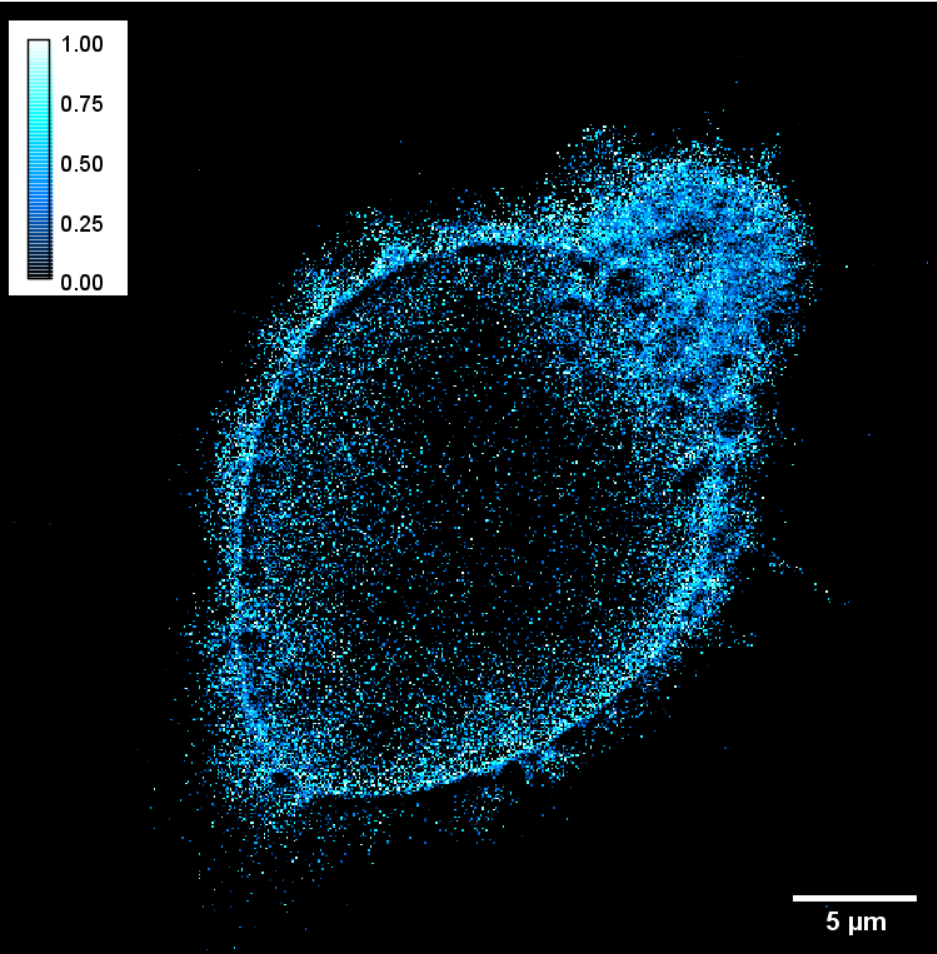
\includegraphics[scale = 0.45]{Bilder/E2.png}
    \caption{2D-Plot der Förstereffizienz $E$ von Zelle 2, pixelweise berechnet.}
    \label{bild:E2}
\end{figure}

\begin{figure}[h]
    \centering
    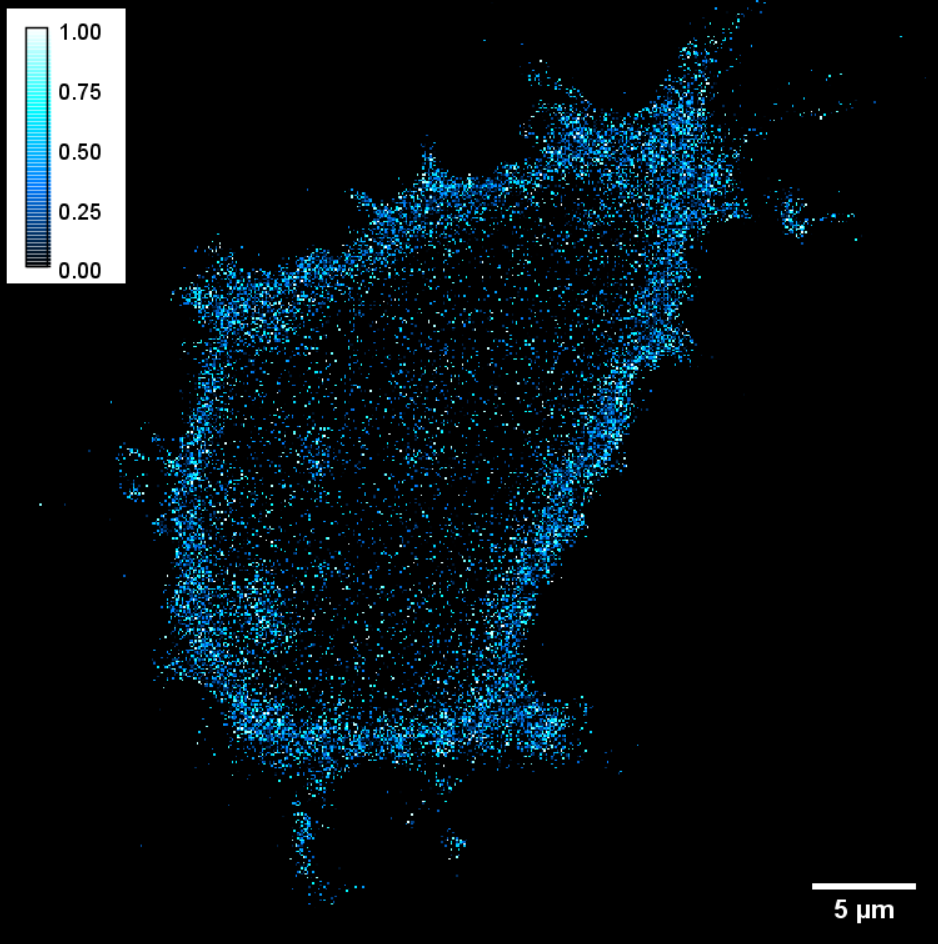
\includegraphics[scale = 0.45]{Bilder/E10.png}
    \caption{2D-Plot der Förstereffizienz $E$ von Zelle 10, pixelweise berechnet.}
    \label{bild:E10}
\end{figure}

\begin{figure}[h]
    \centering
    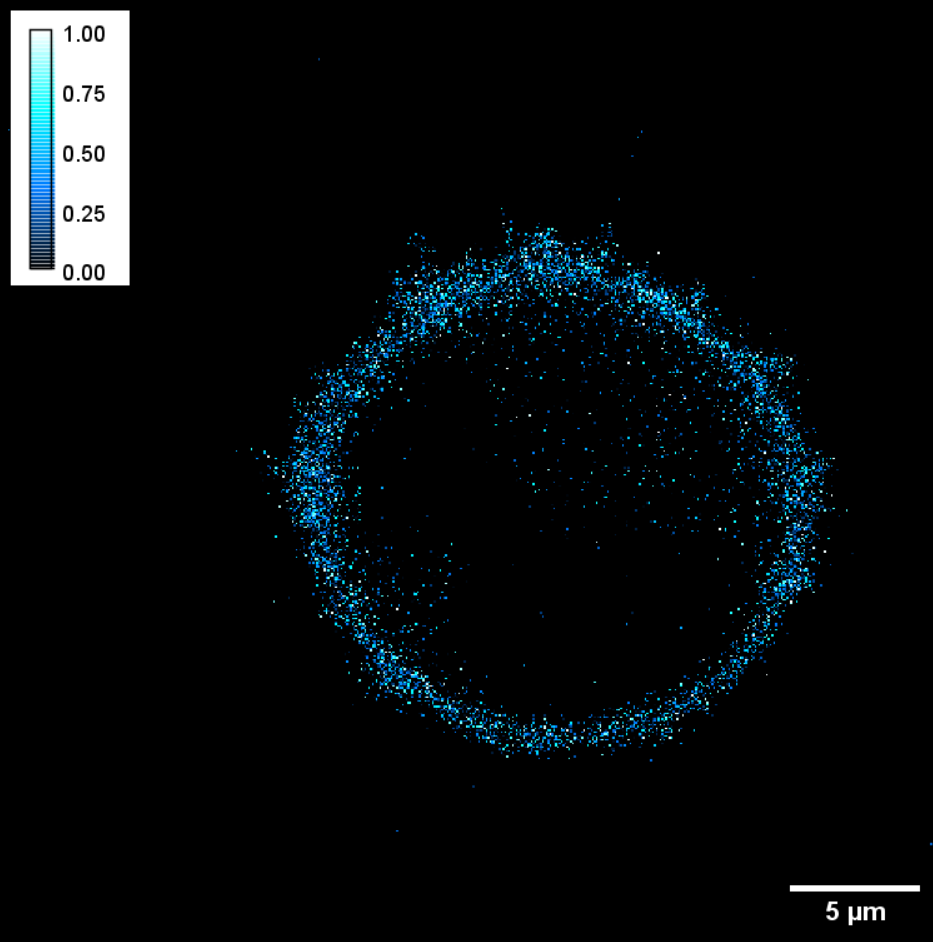
\includegraphics[scale = 0.45]{Bilder/E13.png}
    \caption{2D-Plot der Förstereffizienz $E$ von Zelle 13, pixelweise berechnet.}
    \label{bild:E13}
\end{figure}

\begin{center}
    \centering
    \begin{tabular}{l|r|r}
        Zelle & $E_{aus \, Mittelung}$ & $E_{pixelweise}$\\
        \hline
        2 & 0,379 & 0,413\\
        10 & 0,135 & 0,329\\
        13 & 0,0873 & 0,370\\
    \end{tabular}
    \captionof{table}{Förstereffizienz $E$ für drei ausgewählte Zellen berechnet einmal über die Mittelung der Intensitäten und einmal über die pixelweise Berechnung von $E$ und darauffolgender Mittelung}
    \label{tab:VerglE}
\end{center}

Dabei ist festzustellen, dass die Werte teilweise deutlich voneinander abweichen. Ein gewisser Fehler ist zu erwarten, da es einen Unterschied macht, wo 
genau in der Rechnung gemittelt wird. Ob dieser dennoch so groß ist darf angezweifelt werden. Trotz dessen sind alle Werte für $E$ durchaus 
plausibel.

\clearpage